\documentclass[10pt,xcolor={dvipsnames}]{beamer}
%\usetheme[progressstyle=movingCircCnt,
%%% option passed to the outer theme
%    progressstyle=fixedCircCnt,   % fixedCircCnt, movingCircCnt (moving is deault)
%  ]{Feather}
\usepackage{dbt}

% If you want to change the colors of the various elements in the theme, edit and uncomment the following lines
\usepackage{color, xcolor}

\graphicspath{{figs/}}

%-------------------------------------------------------
% INCLUDE PACKAGES
%-------------------------------------------------------

%%% href
\usepackage[]{hyperref}

\newcommand{\MYhref}[3][blue]{\href{#2}{\color{#1}{#3}}}%
% colored hyperlinks
\newcommand{\chref}[2]{
  \href{#1}{{\color{blue} #2}}
}

\usepackage[utf8]{inputenc}
\usepackage[english]{babel}
\usepackage[T1]{fontenc}

\usepackage{amsmath, amsfonts, amssymb}
\usepackage{mathtools}
% \usepackage{helvet}

%% Load different font packages to use different fonts
%% e.g. using Linux Libertine, Linux Biolinum and Inconsolata
\usepackage{libertine}
% \usepackage{zi4}

\usepackage{qrcode}

%% e.g. using Carlito and Caladea
%\usepackage{carlito}
%\usepackage{caladea}
%\usepackage{zi4}

%% e.g. using Venturis ADF Serif and Sans
% \usepackage{venturis}

%-------------------------------------------------------
% DEFFINING AND REDEFINING COMMANDS
%-------------------------------------------------------

\setmonofont{DejaVu Sans Mono}




% animations
\usepackage{animate}

\usepackage{tikz}
\usepackage{tikz-3dplot}
\usetikzlibrary{calc, fit, positioning}
\usetikzlibrary{arrows}
\usetikzlibrary{shadings,  shadows, shadows.blur}
\usetikzlibrary{shapes, shapes.geometric, shapes.symbols, shapes.arrows}
\usetikzlibrary{automata, snakes, backgrounds, trees, decorations.text}
\usetikzlibrary{decorations, decorations.text}

\usepackage{pgf}
\usepackage{pgfplots}

\usepackage{relsize}


%%%%%%%%%%%%%% important imports
\usepackage{import}
\usepackage{pifont}
\usepackage{minted}




\newcommand\tikzframe[1]{
\begin{tikzpicture}
	\useasboundingbox (current page.north west) rectangle (current page.south east);
	#1
\end{tikzpicture}

}

%-------------------------------------------------------
% INFORMATION IN THE TITLE PAGE
%-------------------------------------------------------

\titlegraphic{
\includegraphics[width=1cm]{sbseg}}

\title
{ % is placed on the title page
      \textbf{Execução de código arbitrário na\\urna eletrônica brasileira}
}

\subtitle
{
      \textbf{SBSeg 2018}
}

\author
{      Diego Aranha (Unicamp), Pedro Barbosa (UFCG),\\
       Thiago Cardoso (Hekima), Caio Lüders (UFPE),\\
       \textbf{Paulo Matias (UFSCar)}\\[1em]
}

\date{}




%-------------------------------------------------------
% THE BODY OF THE PRESENTATION
%-------------------------------------------------------
\usepackage{xmpmulti}

\usepackage{siunitx}
\begin{document}

%-------------------------------------------------------
% THE TITLEPAGE
%-------------------------------------------------------

\begin{frame}[plain,noframenumbering] % the plain option removes the header from the title page, noframenumbering removes the numbering of this frame only
  \titlepage % call the title page information from above
\end{frame}


\begin{frame}{Propriedades de segurança}
Não importando a tecnologia empregada, um sistema de votação precisa satisfazer algumas propriedades:
\begin{enumerate}
 \item \emph{Autenticação dos eleitores}: apenas eleitores autorizados podem votar
 \item \emph{Sigilo do voto}: voto deve ser secreto
 \item \emph{Integridade dos resultados}: resultado é justo
 \item \emph{Possibilidade de auditoria}: idealmente, sem especialização
\end{enumerate}
\end{frame}


\begin{frame}{Um breve histórico}
\begin{enumerate}
 \item[\alert{1996}]: Urnas eletrônicas em 30\% das seções eleitorais
 \item[\alert{2000}]: Primeiras eleições inteiramente eletrônicas
 \item[\alert{2002}]: Primeira experiência com voto impresso
 \item[\alert{2006}]: TSE passa a ser responsável pelo \emph{software}
 \item[\alert{2008}]: Migração para GNU/Linux
 \item[\alert{2009}]: I Testes Públicos de Segurança (quebra de sigilo do voto)
 \item[\alert{2012}]: II TPS (quebra de sigilo do voto)
 \item[\alert{2016}]: III TPS (quebra na integridade de resultados)
 \item[\alert{2017}]: IV TPS (quebra na integridade de \emph{software})
\end{enumerate}
\end{frame}


\begin{frame}{Processo de votação brasileiro}
\begin{center}
\includegraphics[width=\textwidth,height=0.8\textheight,keepaspectratio]{TSE.png}
\end{center}
\end{frame}


\begin{frame}{Instalação (carga) nas urnas}
\begin{center}
\includegraphics[width=\textwidth,height=0.8\textheight,keepaspectratio]{criancas_carga.jpg}
\end{center}
\end{frame}


\begin{frame}{Como funciona o TPS?}
  \begin{itemize}
    \item Fase de inspeção dos códigos fonte
    \item Submetemos \textbf{planos de teste}
    \item TSE analisa e aprova os planos de teste
    \item Executamos os planos de teste em uma bancada com computador e urna eletrônica
  \end{itemize}
\end{frame}


\begin{frame}{Planta do ambiente}
  \begin{center}
  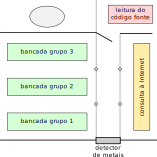
\includegraphics[width=\textwidth,height=0.8\textheight,keepaspectratio]{planta}
  \end{center}
\end{frame}


\begin{frame}{Fase de inspeção dos códigos fonte}
  Encontramos chave da mídia de instalação em claro \\no código fonte do \textit{kernel} 3.18.
  \vfill
  \begin{center}
  \includegraphics[width=\textwidth,height=0.5\textheight,keepaspectratio]{aes-xts-sec.pdf}
  \end{center}
\end{frame}


\begin{frame}{Planos de teste inicialmente submetidos}
  \begin{itemize}
    \item \textbf{QP1}: É possível extrair chaves criptográficas da FC?
    \item \textbf{QP2}: É possível violar o sigilo do voto explorando o gerador de números
pseudo-aleatórios?
    \item \textbf{QP3}: É possível inserir um dispositivo USB malicioso na urna?
    \item \textbf{QP4}: É possível executar código remoto na plataforma \textit{web} de totalização?
  \end{itemize}
\end{frame}


\begin{frame}[fragile]{Chave encontrada no \textit{kernel}: um atalho}
\begin{minted}[fontsize=\smaller]{python}
class Codebook:
    def __init__(self, key):
        self.key = key

    def aes(self, key, block, mode='-d'):
        if mode == '-d':
            block += block  #need 256 bits to work with
                            #the command below
        p = Popen(['openssl','enc','-aes-256-ecb',mode,
                   '-K',key.encode('hex')],
                  stdin=PIPE,stdout=PIPE,
                  stderr=open('/dev/null','w'))
        p.stdin.write(block)
        p.stdin.close()
        return p.stdout.read()[:16] #but we ignore the last 128 bits

    def decrypt(self, block):
        return self.aes(self.key, block, '-d')

    def encrypt(self, block):
        return self.aes(self.key, block, '-e')
\end{minted}
\end{frame}


\begin{frame}{Inspeção da cadeia de confiança}
\begin{center}
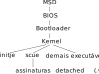
\includegraphics[width=\textwidth,height=0.5\textheight,keepaspectratio]{assinaturas_sistema.pdf}
\end{center}
\end{frame}


\begin{frame}{Elo fraco: assinaturas separadas}
\begin{center}
\includegraphics[width=\textwidth,height=0.5\textheight,keepaspectratio]{assinaturas_sistema_weak_link.pdf}
\end{center}
\end{frame}


\begin{frame}{Elo fraco: assinaturas separadas}
  \begin{itemize}
    \item Ausência de assinatura das bibliotecas \textbf{libhkdf.so} e \textbf{libapilog.so} nos arquivos de assinaturas separadas (VST).
    \item Interferir com código do SCUE por meio de bibliotecas ligadas a este permitiria contornar totalmente VSTs, pois o \textit{kernel} só verificava o binário principal.
    \vfill
    \item Introdução da \textbf{QP5}: É possível executar código arbitrário na\\urna eletrônica?
    \item Tempo restrito: equipe decidiu deixar de investigar \textbf{QP2--4}.
  \end{itemize}
\end{frame}


\begin{frame}{Execução arbitrária de código}
  \textbf{Método}: Alterar \textbf{libhkdf.so} ou \textbf{libapilog.so} para injetar código malicioso.
  \vfill

  Diversas demonstrações dando suporte a \textbf{QP5}:

  \begin{itemize}
    \item Imprimir \alert{``\texttt{FRAUDE!}''} durante a inicialização da urna.
    \item Manipular \textit{log} para mostrar \alert{``\texttt{XXXX}''} em vez de \alert{``\texttt{INFO}''}.
    \item Quebrar o sigilo do voto, por meio de mudança da chave do\\registro digital do voto (RDV), permitindo contar votos antes e depois de um eleitor entrar na seção:\\[0.5em]

    \texttt{[98, 99, null, \alert{null}]} $\rightarrow$ \texttt{[98, 99, null, \alert{99}]}

    \item Interferir sobre páginas de memória somente leitura:\\\alert{``\texttt{A Hora da Estrela}''} $\rightarrow$ \alert{``\texttt{A Hora da Treta}''}.
  \end{itemize}
\end{frame}


\begin{frame}{Demonstração: interferir sobre a interface gráfica}
\begin{center}
\includegraphics[width=\textwidth,height=0.5\textheight,keepaspectratio]{tela-adulterada.png}
\end{center}
\end{frame}


\begin{frame}[fragile]{Demonstração: interferir com armazenamento dos votos}
  \textbf{Método}: Alterar código do método \alert{\texttt{\small void \textbf{AdicionaVoto}(uint8\_t cargo, int tipo, std::string \&voto)}}, da classe \alert{\texttt{\small InfoEleitor}} do aplicativo de votação.

  \vfill
  \begin{itemize}
    \item Inserir uma instrução \alert{\texttt{ret}} causou erro de asserção (tamanho do \texttt{\small std::vector} da cédula deveria ser diferente de zero) apenas depois de pressionado \textcolor{green}{``Confirma''}.\\[1em]

    \item Código para desvio de votos obteve sucesso em um simulador de urna:\\[0.5em]
    \begin{minted}[fontsize=\smaller]{nasm}
mov eax, [ebp+0x14]  ; std::string&
mov edi, [eax]       ; char*
mov al, '9'
stosb
stosb
    \end{minted}
  \end{itemize}
\end{frame}


\begin{frame}{Término do TPS 2017}
  \begin{itemize}
    \item Grupo da Polícia Federal deu suporte à \textbf{QP1} (É possível extrair chaves criptográficas da FC), obtendo a chave do sistema de arquivos por meio de extração da memória de uma máquina virtual.
    \item Análise superficial da \textbf{QP2} (É possível violar o sigilo do voto explorando o gerador de números pseudo-aleatórios?): urna utiliza variante do gerador Sapparot-2 (não criptográfico) intercalado com gerador do Linux.
    \item Demos suporte à \textbf{QP5} (É possível executar código arbitrário na
urna eletrônica) por meio de diversas demonstrações.
  \end{itemize}
\end{frame}


\begin{frame}{Contramedidas adotadas pelo TSE}
  \begin{itemize}
    \item Uso de trecho da Flash da BIOS como chave para cifrar a mídia.\\
        {\small \alert{Limitação}: Flash da BIOS pode ser extraída por um atacante uma única vez, de qualquer urna do país.}\\[1em]
    \item Compilação de binários PIE.\\
        {\small \alert{Limitação}: Endereços podem ser calculados a partir de informações\\contidas na pilha.}\\[1em]
    \item Inclusão de todos os arquivos nos VSTs.\\
        {\small \alert{Limitação}: Verificação pode ser desabilitada interferindo-se com SCUE.}\\[1em]
    \item Ligação estática com libapilog, libhkdf, \textit{etc.}\\
        {\small \alert{Limitação}: A libc poderia ser infectada.}\\[1em]
    \item Verificação de assinatura de bibliotecas pelo \textit{kernel}.\\
        {\small \alert{Limitação}: Cadeia de confiança complexa, muito código customizado.\\É difícil atestar que não existem outras falhas.}
  \end{itemize}
\end{frame}


\begin{frame}{Conclusão}
  Recomenda-se ao TSE:
  \begin{itemize}
    \item Reduzir a burocracia e ampliar escopo e duração dos testes.
    \item Revisar práticas internas de desenvolvimento.
    \item Considerar novamente a introdução de um registro físico do voto.
  \end{itemize}
\end{frame}

\begin{frame}{Mais informações em}
  \begin{minipage}{.485\linewidth}
  \begin{center}
      \fcolorbox{gray}{white}{\textcolor{black}{\qrcode[height=4cm]{https://github.com/epicleet/tps2017}}}\\[1em]\scriptsize\url{https://github.com/epicleet/tps2017}
  \end{center}
  \end{minipage}
  \hfill
  \begin{minipage}{.485\linewidth}
  \begin{center}
      \fcolorbox{gray}{white}{\textcolor{black}{\qrcode[height=4cm]{https://urnaeletronica.info}}}\\[1em]\scriptsize\url{https://urnaeletronica.info}
  \end{center}
  \end{minipage}
\end{frame}

\end{document}
